\icode[magenta]{E-MCC-CA-L4-260626-001}
如图所示在足够大的转盘中心固定一个小物块B，距离中心为\(r_0 =\)\qty{0.2}{m}处放置小物块\(A\)，\(A\)、\(B\)质量均为\(m =\)\qty{1}{kg}，\(A\)与转盘之间的动摩擦因数为\(\mu_1 = 0.5\)，现在用原长为\(d =\) \,\qty{0.2}{m}、劲度系数\(k =\)\qty{40}{N/m}的轻质弹簧将两者拴接，重力加速度\(g =\)\qty{10}{m/s^2}，假设弹簧始终处于弹性限度以内，最大静摩擦力等于滑动摩擦力，则：
\begin{enumerate}
    \item 缓慢增加转盘转动的角速度，求\(A\)即将打滑时的\(\omega_0\)；
    \item 若转盘的角速度\(\omega_1 =\)\qty{6}{rad/s}，\(A\)可以放置在离中心距离不同的位置上，且\(A\)始终不打滑，求满足条件的\(A\)转动半径\(r_A\)的大小范围；
    \item 若小物块\(B\)解除固定状态，\(B\)和转盘间动摩擦因数为\(\mu_2 = 0.2\)，现将转盘角速度从0开始缓慢增大，为了保证\(B\)不打滑，求满足条件的转盘角速度\(\omega_2\)的大小范围。
\end{enumerate}

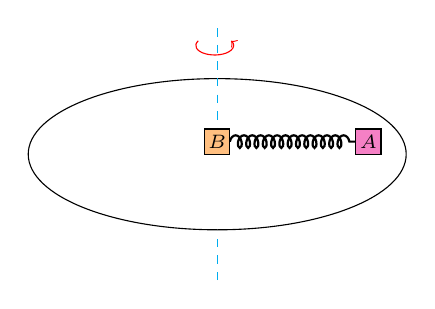
\begin{tikzpicture}[scale=.8,font=\scriptsize]
    \draw[dashed,cyan] (0,-2)--(0,0);
    \draw[fill=white] (0,0) ellipse(3 and 1.2);
    \draw[dashed,cyan] (0,2)--(0,0);
    \draw[thick,decoration={aspect=.6,segment length=3,amplitude=.8mm,coil},decorate] (.2,.2)--(2.2,.2);
    \draw[fill=orange!50] (-.2,0) rectangle(.2,.4)node[pos=.5]{\(B\)};
    \draw[fill=magenta!50] (2.2,0) rectangle(2.6,.4)node[pos=.5]{\(A\)};
    \draw[->,red] (-.3,1.8) arc(-210:30:.3 and .15);
\end{tikzpicture}